\documentclass{article}
\usepackage{fancyhdr}
\usepackage{titlesec}
\usepackage{graphicx}
\graphicspath{ {./img/} }

\pagestyle{fancy}
\fancyhf{}
\lhead{Modul 2 Praktikum Jaringan Komputer}
\rfoot{\footnotesize Page \thepage}
\lfoot{\footnotesize Mahyus Ihsan, S.Si, M.Si \newline Jurusan Informatika Universitas Syiah Kuala \newline Modul oleh : Diky Wahyudi, Furqan Al Ghifari, Rendika Rahmaturrizki}
\renewcommand{\headrulewidth}{1pt}
\renewcommand{\footrulewidth}{1pt}

\titleformat*{\section}{\small\bfseries}

\begin{document}
    \begin{center}
        \textbf{Modul 2 Praktikum Jaringan Komputer}

        \textbf{Protocol, Models dan Ethernet Switching}
    \end{center}

    \section*{Deskripsi Singkat}
    Protokol jaringan komputer adalah aturan yang ada dalam sebuah jaringan komputer yang harus ditaati oleh pihak pengirim dan penerima agar dapat saling berkomunikasi dan bertukar informasi meskipun memiliki sistem yang berbeda. Model adalah beberapa model dari protokol jaringan. Dan Ethernet Switching adalah cara internet bekerja dalam komunikasi jaringan.

    \section*{Tujuan}
    \begin{enumerate}
        \item Dapat memahami berbagai macam protokol jaringan beserta modelnya.
        \item Dapat memahami cara kerja protokol dalam melakukan komunikasi.
        \item Dapat memahami cara kerja dan struktur pada ethernet.
    \end{enumerate}

    \begin{flushleft}
        \textbf{Materi 1 - Protocol dan Model}
        \newline

        Untuk bisa berkomunikasi antar perangkat ada aturan yang harus ditetapkan dan aturan tersebut adalah protokol. Protokol pada jaringan terbagi berbagai macam tipe :

        \begin{description}
            \item[Network Communications Protocols] adalah protokol yang berfungsi untuk komunikasi antar perangkat ataupun jaringan. 
            Protokol yang termasuk NCP adalah Internet Protocol (IP), Transmission Control Protocol (TCP), HyperText Transfer Protocol (HTTP) dan lain-lain.
            \item[Network Security Protocols] adalah protokol yang berfungsi untuk keamanan data, integrasi data , autentikasi dan enkripsi data. 
            Protokol yang termasuk NSP adalah Secure Shell (SSH), Secure Sockets Layer (SSL), dan Transport Layer Security (TLS).
            \item[Routing Protocols] adalah protokol yang berfungi untuk komunikasi antar router agar dapat mencari rute ke alamat yang dituju dengan waktu yang tersingkat. 
            Protokol yang termasuk Routing Protocol adalah Open Shortest Path First (OSPF) dan Border Gateway Protocol (BGP).
            \item[Service Discovery Protocols] adalah protokol yang digunakan dalam mendeteksi perangkat atau jaraingan secara otomatis.
            Protokol yang termasuk SDP adalah  Dynamic Host Configuration Protocol (DHCP) dan Domain Name System (DNS).
        \end{description}

        Dalam modul kali ini protokol yang akan di bahas adalah model TCP/IP dan model OSI layer.

        Perbandingan model dari OSI Layer dan TCP/IP layer.
        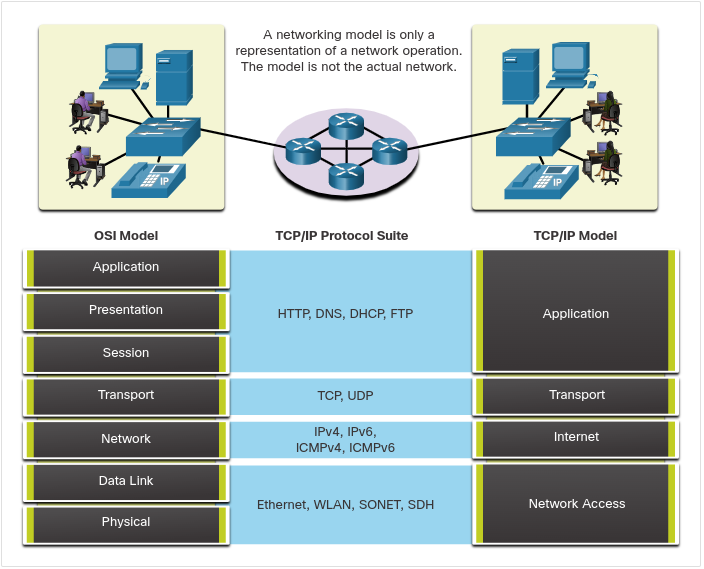
\includegraphics[scale=0.65]{osi-tcp-layer.png}

        \textbf{Layer pada OSI model.}
        \begin{itemize}
            \item[] \textbf{Layer 7 - Application Layer}
            \newline
            Berfungsi sebagai antarmuka dengan aplikasi dengan fungsionalitas jaringan, mengatur bagaimana aplikasi dapat mengakses jaringan, dan kemudian membuat pesan-pesan kesalahan.

            \item[] \textbf{Layer 6 - Presentation Layer}
            \newline
            Berfungsi untuk mentranslasikan data yang hendak ditransmisikan oleh aplikasi ke dalam format yang dapat ditransmisikan melalui jaringan.

            \item[] \textbf{Layer 5 - Session Layer}
            \newline
            Berfungsi untuk mendefinisikan bagaimana koneksi dapat dimulai, dipelihara, atau diakhiri.

            \item[] \textbf{Layer 4 - Transport Layer}
            \newline
            Berfungsi untuk memecah data ke dalam paket-paket data serta memberikan nomor urut ke paket-paket tersebut sehingga dapat disusun kembali pada sisi tujuan setelah diterima.

            \item[] \textbf{Layer 3 - Network Layer}
            \newline
            Berfungsi untuk mendefinisikan alamat-alamat IP dan menyediakan fungsi routing sehingga paket dapat dikirim keluar dari segment network lokal ke suatu tujuan yang berada pada suatu network lain.

            \item[] \textbf{Layer 2 - Data Link Layer}
            \newline
            Berfungsi untuk menentukan bagaimana bit-bit data dikelompokkan menjadi format yang disebut sebagai frame.

            \item[] \textbf{Layer 1 - Physical Layer}
            \newline
            berfungsi untuk mendefinisikan media transmisi jaringan, sinkronisasi bit, arsitektur jaringan (seperti Ethernet), topologi jaringan dan pengabelan.
        \end{itemize}

    \end{flushleft} 

    \begin{flushleft}
        \textbf{Materi 2 - Simulasi OSI model dengan menggunakan Packet Tracer}
        \newline

        \begin{enumerate}
            \item Download package cisco yang terdapat pada \textbf{ CiscoPacket.zip}
            \newline
            \textbf{3.5.5-packet-tracer---investigate-the-tcp-ip-and-osi-models-in-action.pka}

            \item Buka package tersebut menggunakan Packet Tracer
            \newline
            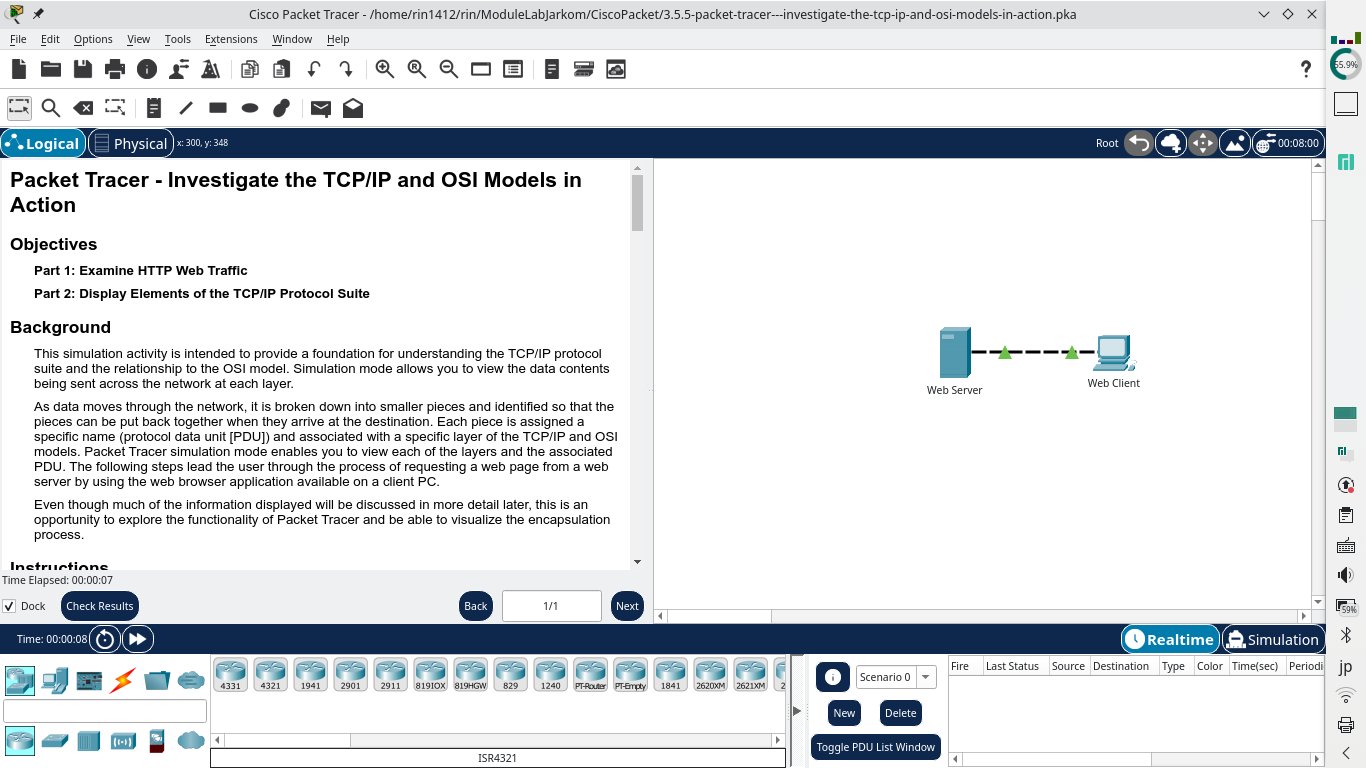
\includegraphics[scale=0.3]{2-open-packet.png}

            \item Klik dua kali pada komputer \textbf{Web Client}, kemudian masuk ke dalam menu \textbf{Desktop} dan buka aplkasi \textbf{Web Browser}. Pada aplikasi web browser ketikkan \textbf{\textit{www.osi.local}} pada kolom URL dan kemudian klik tombol \textbf{Go}.
            \newline
            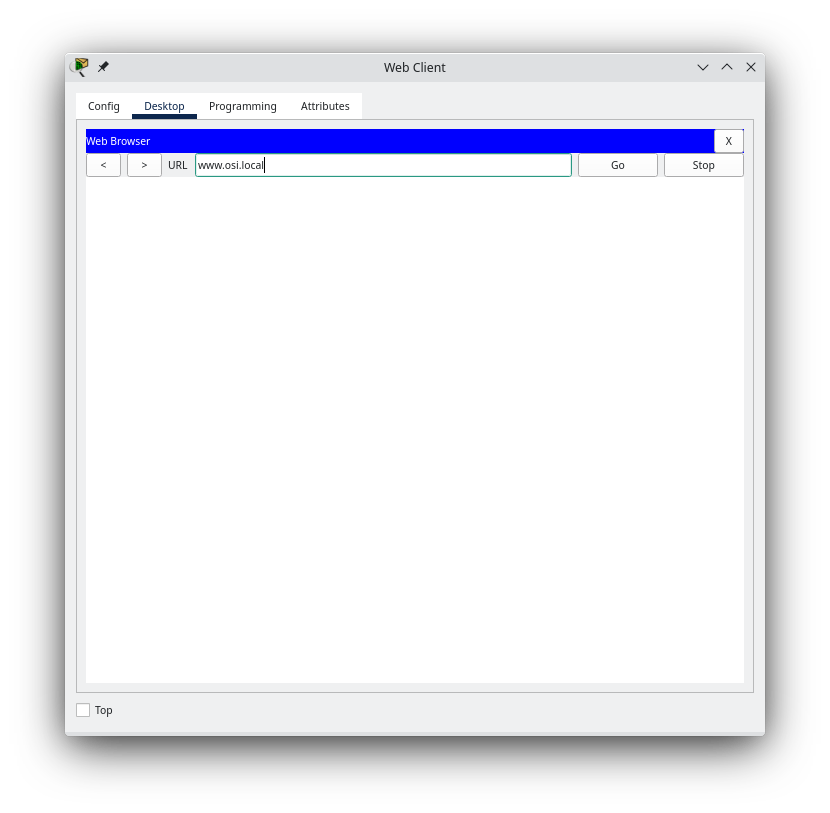
\includegraphics[scale=0.5]{2-open-broswer.png}

            \item Lalu pada packet tracer pilih menu \textbf{Simulation} dan pada bagian \textbf{Play Controls} klik tombol \textbf{Play}. Apa yang terjadi antara Web Client dan Web Server ?
            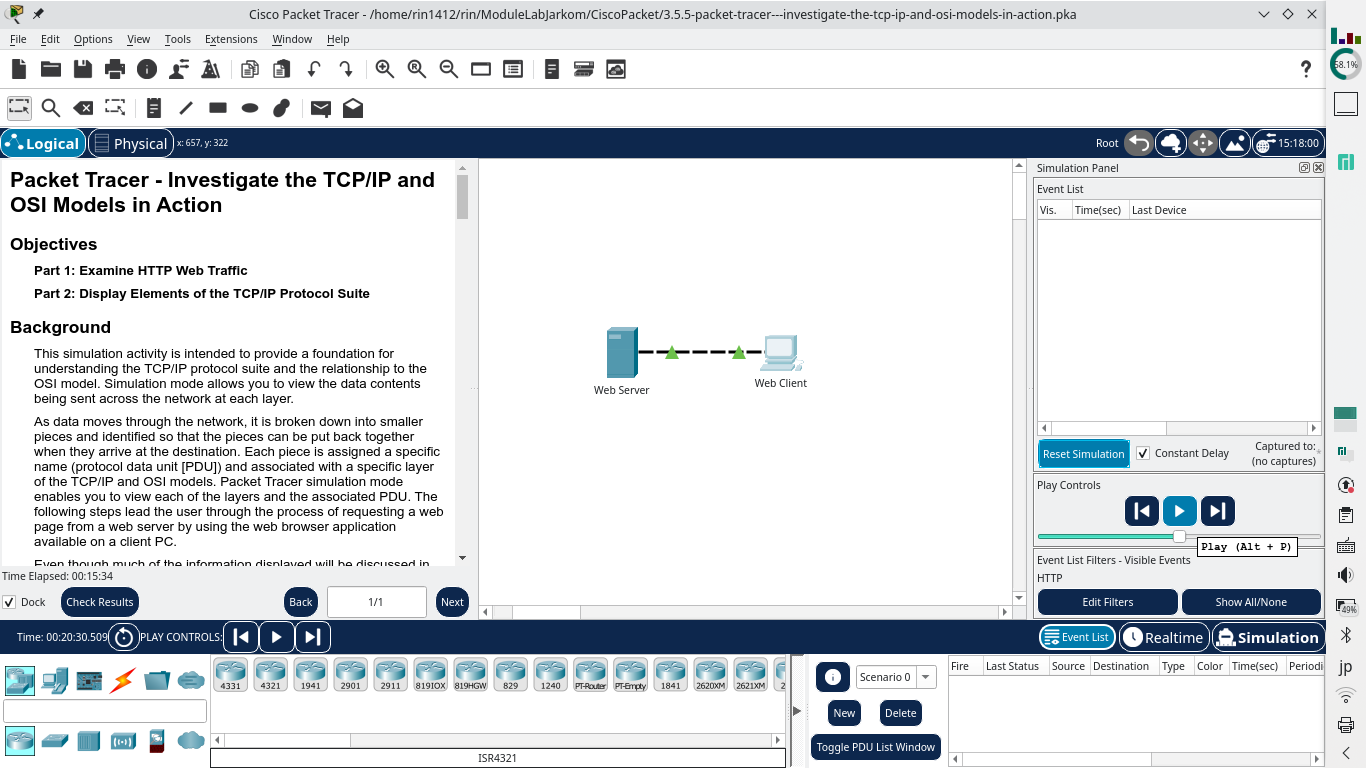
\includegraphics[scale=0.3]{2-play-simulation.png}
            \newline

            \item Pada panel simulasi, pilih salah satu dari langkah-langkah yang terjadi pada saat komunikasi terjadi. Maka akan tampil OSI layer yang di lalui pada masing-masing perangkat pada saat komunikasi terjadi.
            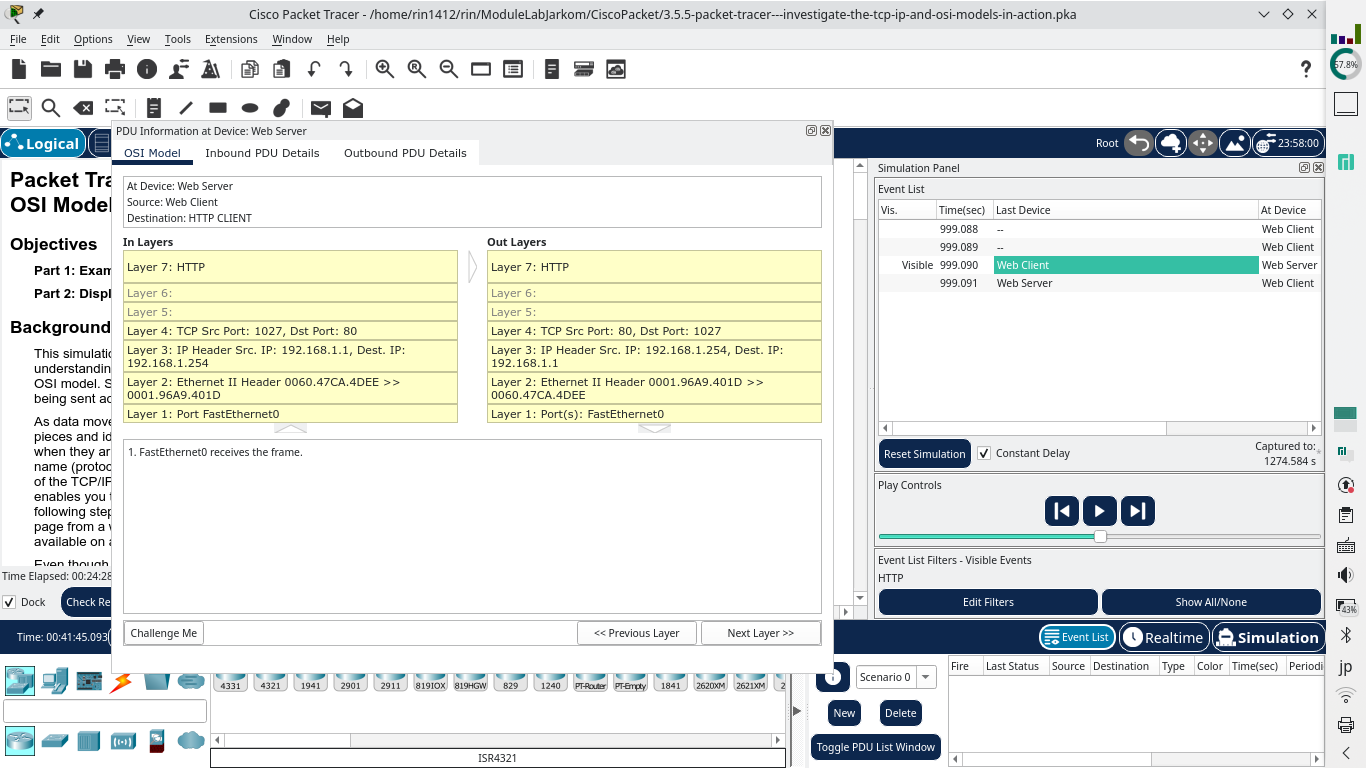
\includegraphics[scale=0.3]{2-osi-layer-sim.png}
        \end{enumerate}
    \end{flushleft}

    \begin{flushleft}
        \textbf{Materi 3 - Ethernet Switching}
        \newline

        \textbf{Ethernet Switching} terletak pada layer 1 dan layer 2 pada OSI model.
        Lebih tepatnya \textbf{Ethernet Switching} terletak pada \textit{Physical Layer dan Data Link Layer}.
        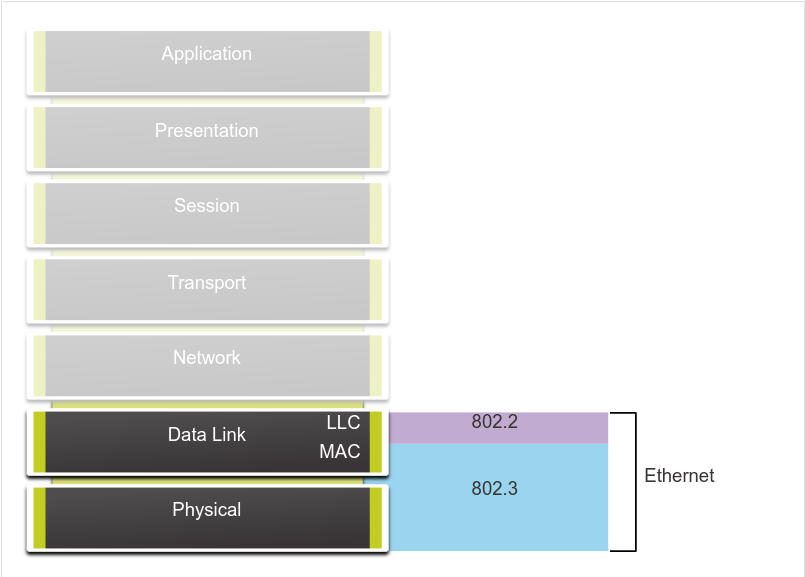
\includegraphics[scale=0.5]{3-ethernet-layer.png}

        Pada \textit{Data Link Layer} terdapat dua sub-layer yaitu Logical Link Control (LLC) dan Media Access Control (MAC).
        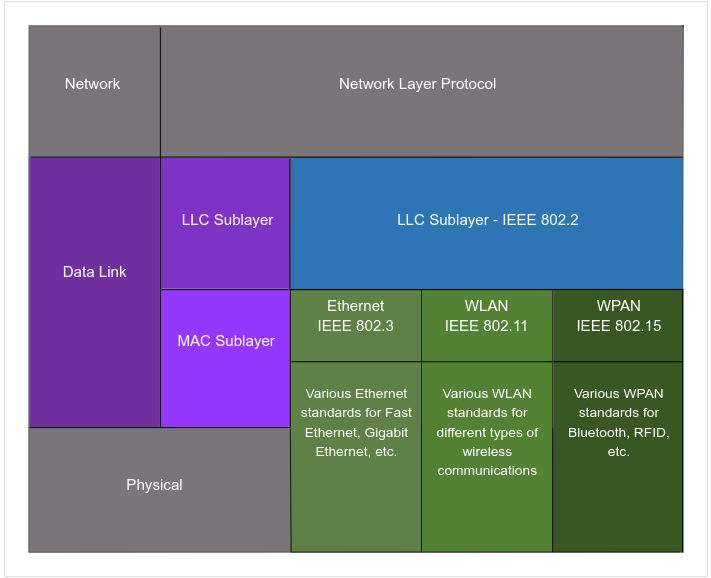
\includegraphics[scale=0.6]{3-llc-mac.png}

        Pada MAC sub-layer terdapat \textbf{Ethernet Frame Fields} atau \textbf{Enkapsulasi Paket Data} yang berfungsi untuk memberi keterangan tentang paket yang akan di kirim.
        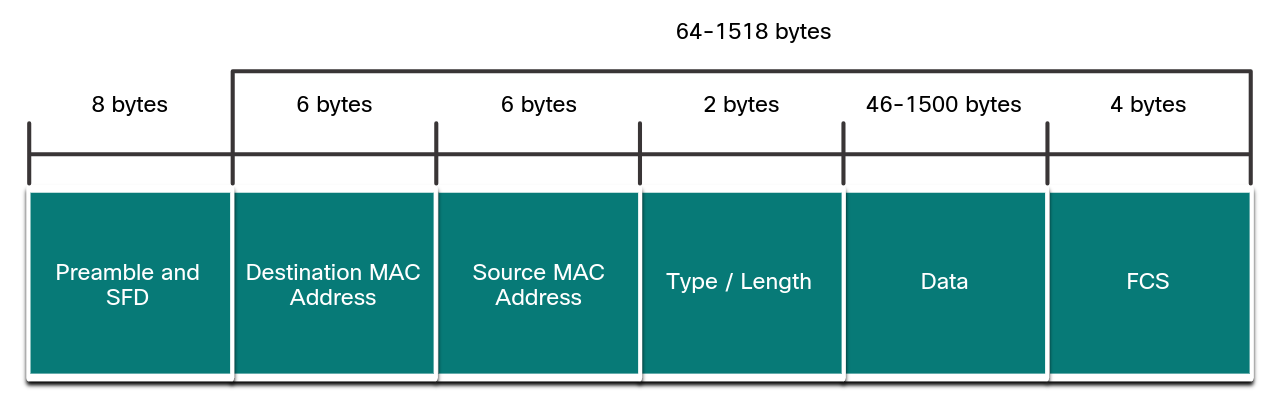
\includegraphics[scale=0.35]{3-mac-frame.png}

        Pada simulasi \textbf{Ethernet Frame Fields} bisa menggunakan percobaan pada materi 2 sebelumnya.
        Pada langkah ke-lima untuk menampilkan OSI layer, silahkan pilih menu \textbf{Inbound PDU Details} atau \textbf{Outbound PDU Details}
        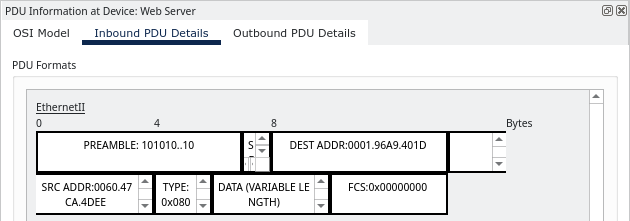
\includegraphics[scale=0.6]{3-mac-frame-eth-0.png}

        Pada bagian Ethernet terdapat \textbf{Ethernet Frame Fields} yang berisi tentang paket yang akan dikirimkan. 
        Sedangkan pada bagian IP berisi tentang pengalamatan dan perutean, serta muatan untuk data. Header TCP terdiri dari beberapa field yang memiliki fungsi yang berbeda. TCP menggunakan header untuk manajemen koneksi, pemutusan koneksi, dan transfer data. Ukuran dari header TCP bervariasi.
        \newline
        
        Header IP \newline
        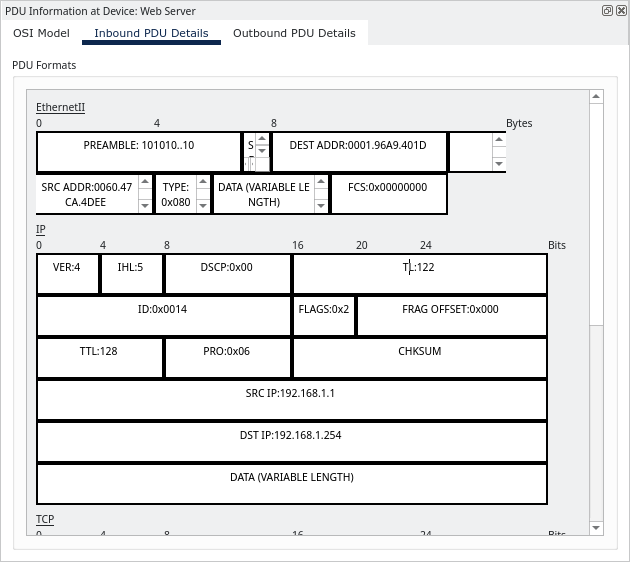
\includegraphics[scale=0.5]{3-mac-frame-eth.png}

        Header TCP \newline
        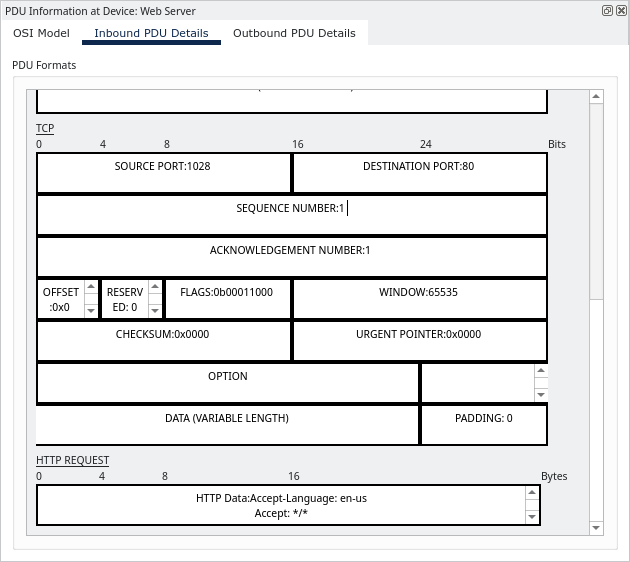
\includegraphics[scale=0.5]{3-mac-frame-tcp.png}
    \end{flushleft}
\end{document}
